% !TEX TS-program = pdflatex
% !TEX encoding = UTF-8 Unicode

\documentclass{beamer}
% for handouts: \documentclass[handout]{beamer}

%\setbeamertemplate{background canvas}[vertical shading][bottom=white,top=structure.fg!25]
% or whatever

\usetheme[compress]{Amsterdam}
%\setbeamertemplate{headline}{}
%\setbeamertemplate{footline}{}
%\setbeamersize{text margin left=0.5cm}
  
\usepackage[english]{babel}
\usepackage{listings}
\usepackage{geometry}
\usepackage{hyperref}
\usepackage{multicol}


\usepackage[utf8]{inputenc}
\usepackage[T1]{fontenc}
\usepackage{lmodern}

\lstset{
basicstyle=\scriptsize\ttfamily,
columns=flexible,
breaklines=true,
numbers=left,
numberstyle=\tiny,
backgroundcolor=\color[rgb]{0.85,0.90,1}
}


\begin{document}

\title[Automated Content Analysis with Python]{\textbf{Four-day workshop\\ Automated Content Analysis with Python} \\ Day 4}
\author[Damian Trilling]{Damian Trilling \\ ~ \\ \footnotesize{d.c.trilling@uva.nl \\@damian0604} \\ \url{www.damiantrilling.net}}
\date{26--9--2017}
\institute[UvA]{Afdeling Communicatiewetenschap \\Universiteit van Amsterdam}

%\maketitle
\begin{frame}{}
\titlepage
\end{frame}

\begin{frame}{Today}
\tableofcontents
\end{frame}

%{\setbeamercolor{background canvas}{bg=black}
%\begin{frame}[plain]
%\makebox[\linewidth]{
%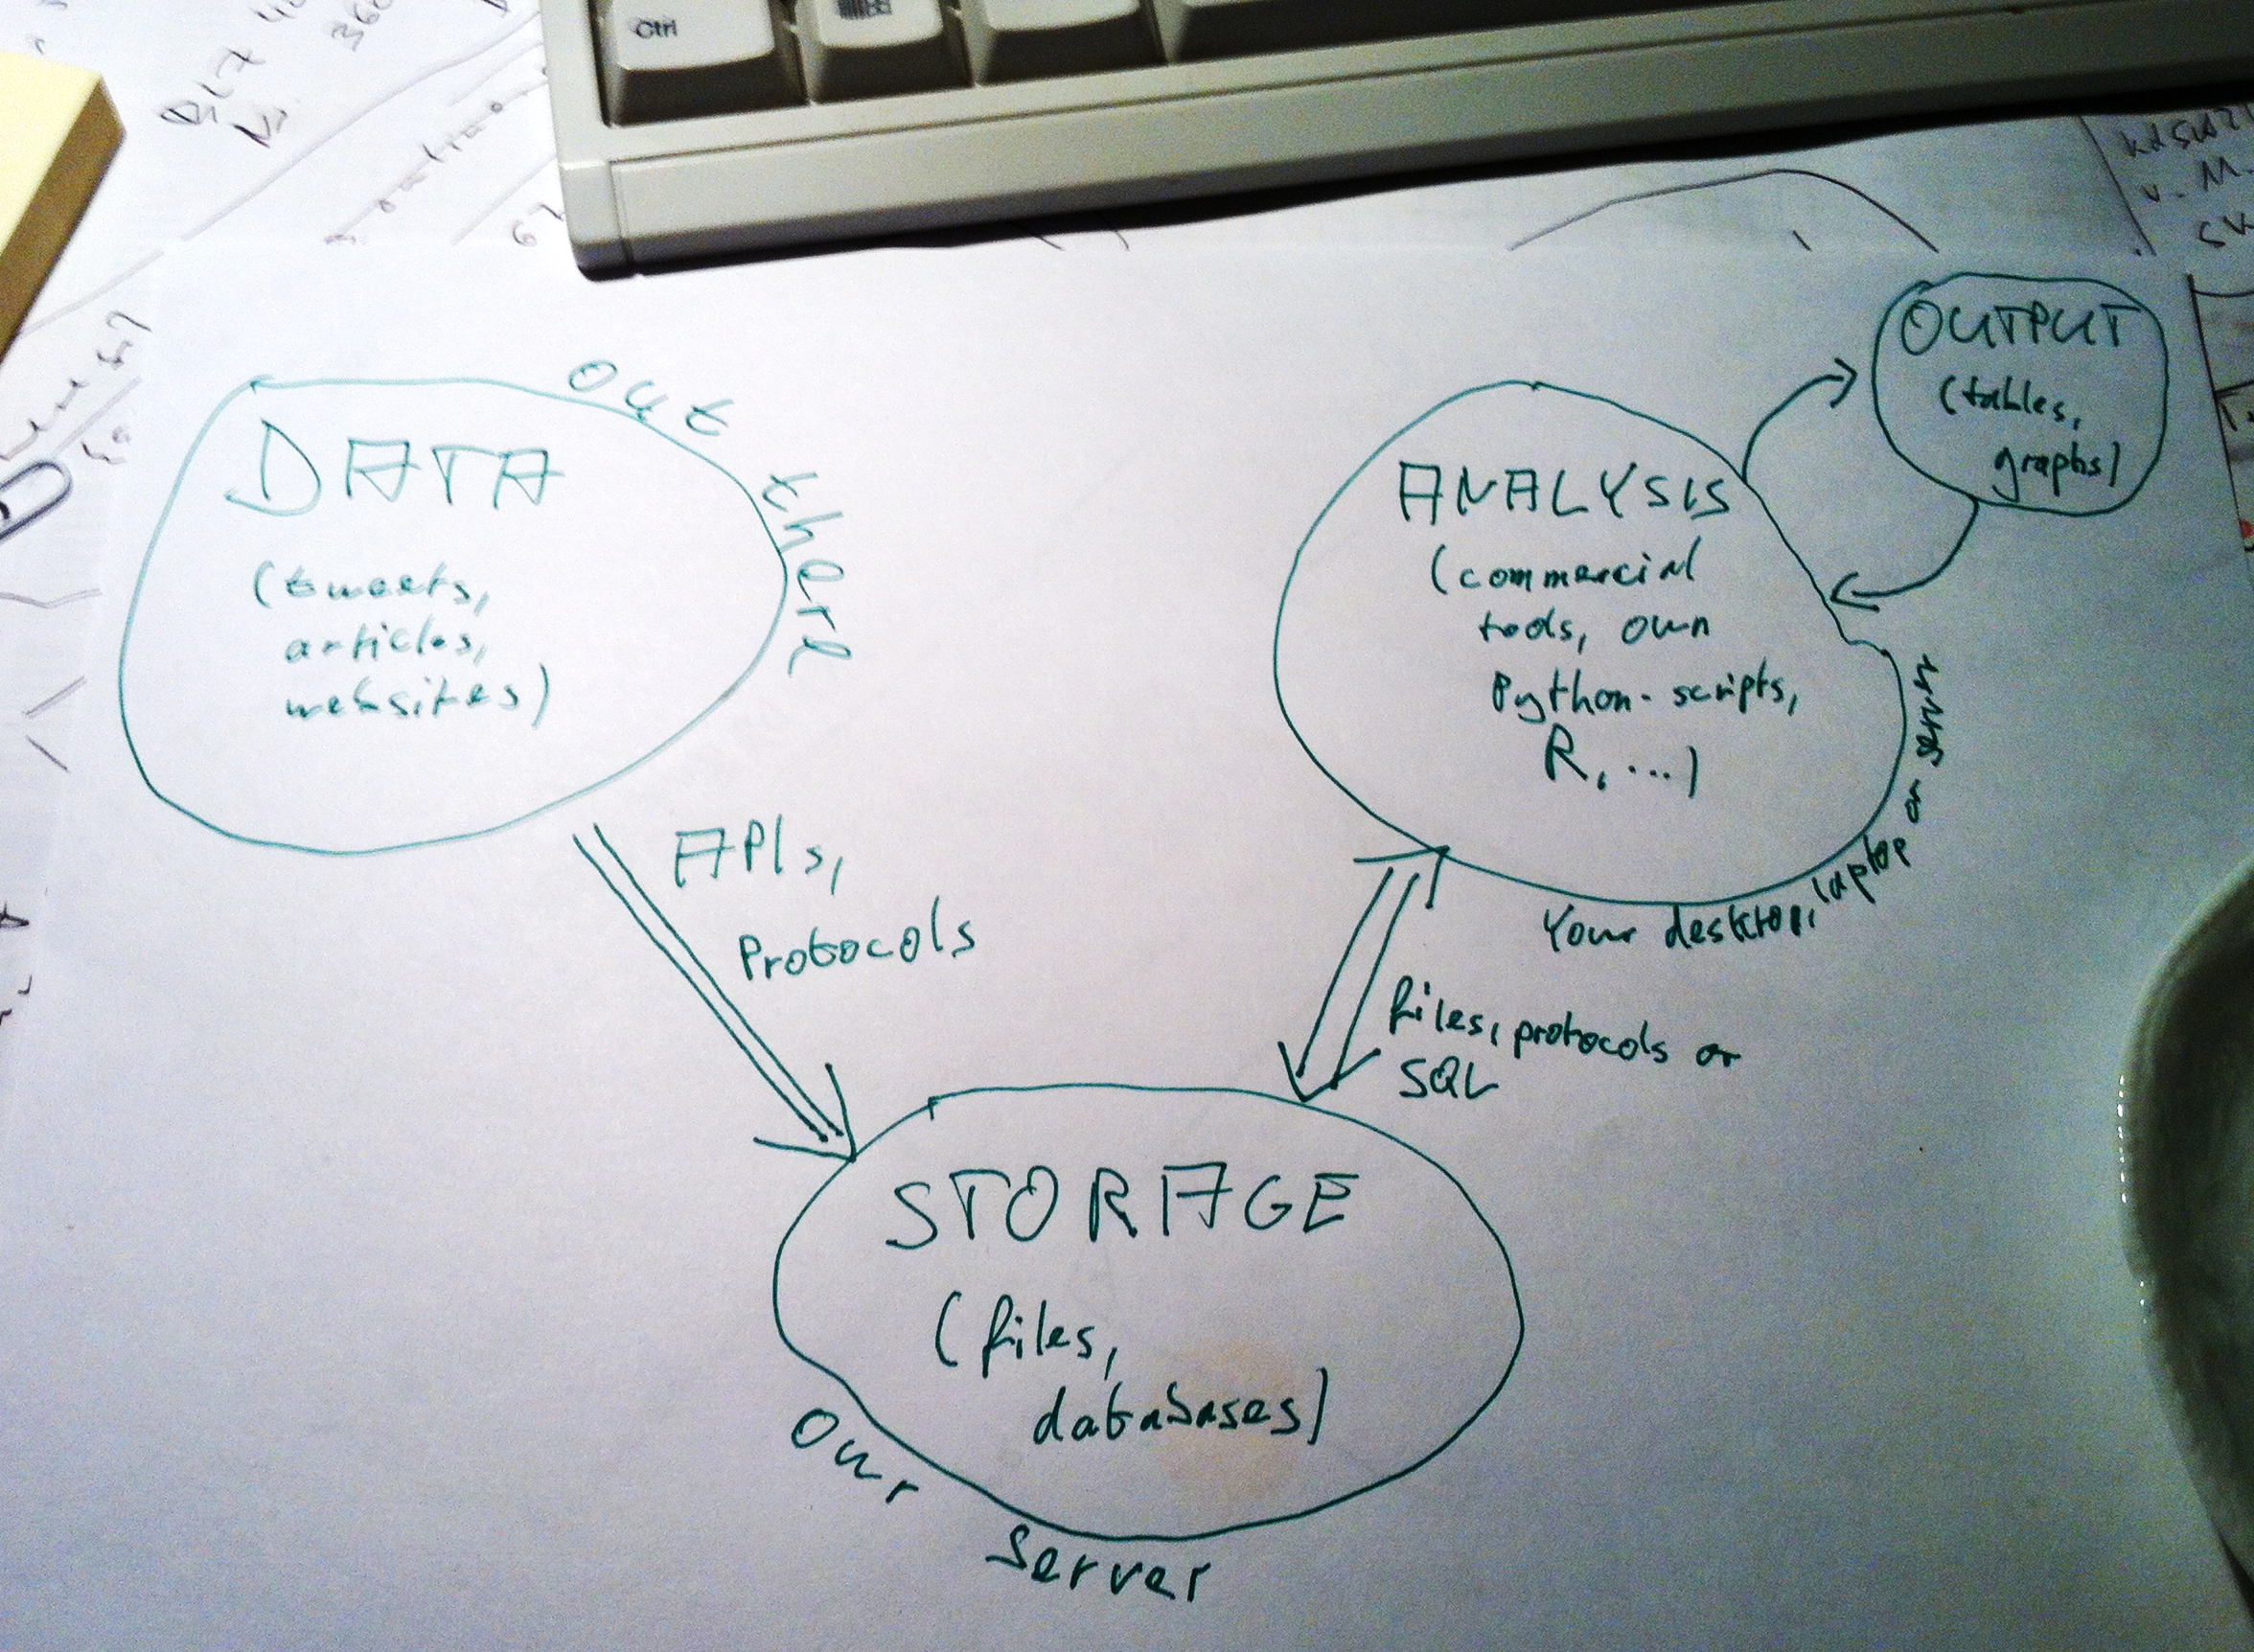
\includegraphics[width=\paperwidth,height=\paperheight,keepaspectratio]{process-heel.png}}
%\end{frame}
%}


\section[Magic Cap]{We put on our magic cap, pretend we are Firefox, scrape all comments from GeenStijl, clean up the mess, and put the comments in a neat CSV table}

\begin{frame}
We put on our magic cap, pretend we are Firefox, scrape all comments from GeenStijl, clean up the mess, and put the comments in a neat CSV table
\end{frame}


{\setbeamercolor{background canvas}{bg=black}
\begin{frame}[plain]
\makebox[\linewidth]{
\includegraphics[width=\paperwidth,height=\paperheight,keepaspectratio]{geenstijl.png}}
\end{frame}
\begin{frame}[plain]
\makebox[\linewidth]{
\includegraphics[width=\paperwidth,height=\paperheight,keepaspectratio]{geenstijl_detail.png}}
\end{frame}
%\begin{frame}[plain]
%\makebox[\linewidth]{
%\includegraphics[width=\paperwidth,height=\paperheight,keepaspectratio]{../plaatjes/geenstijl_sourcecode.png}}
%\end{frame}
\begin{frame}[plain]
\makebox[\linewidth]{
\includegraphics[width=\paperwidth,height=\paperheight,keepaspectratio]{geenstijl_sourcecode_detail.png}}
\end{frame}
}


\begin{frame}{Let's make a plan!}
\begin{block}{Which elements from the page do we need?}
\begin{itemize}
\item What do they mean?
\item How are they represented in the source code?
\end{itemize}
\end{block}
\begin{block}{How should our output look like?}
\begin{itemize}
\item What \emph{lists} do we want?
\item \ldots
\end{itemize}
\end{block}
And how can we achieve this?
\end{frame}


\begin{frame}{}
\begin{block}{Operation Magic Cap}
\begin{enumerate}
\item<2-> Download the page
   \begin{itemize}
   \item<3-> They might block us, so let's do as if we were a web browser!
   \end{itemize}
\item<4-> Remove all line breaks (\textbackslash n, but maybe also \textbackslash n\textbackslash r or \textbackslash r) and TABs (\textbackslash t): We want one long string
\item<5-> Isolate the comment section (it started with {\tt{<div class="commentlist">}} and ended with {\tt{</div>}})
\item<6-> Within the comment section, identify each comment ({\tt{<article>}})
\item<7-> Within each comment, seperate the text ({\tt{<p>}}) from the metadata {\tt{<footer>}})
\item<8-> Put text and metadata in lists and save them to a csv file
\end{enumerate}
\end{block}
\onslide<9->{\textbf{And how can we achieve this?}}
\end{frame}

\begin{frame}[fragile,plain]
\begin{lstlisting}
from urllib import request
import re
import csv

onlycommentslist=[]
metalist=[]

req = request.Request("http://www.geenstijl.nl/mt/archieven/2014/05/das_toch_niet_normaal.html", headers={"User-Agent" : "Mozilla/5.0"})
tekst=request.urlopen(req).read()
tekst=tekst.decode(encoding="utf-8",errors="ignore").replace("\n"," ").replace("\t"," ")

commentsection=re.findall(r'<div class="commentlist">.*?</div>',tekst)
print (commentsection)
comments=re.findall(r'<article.*?>(.*?)</article>',commentsection[0])
print (comments)
print ("There are",len(comments),"comments")
for co in comments:
    metalist.append(re.findall(r'<footer>(.*?)</footer>',co))
    onlycommentslist.append(re.findall(r'<p>(.*?)</p>',co))
writer=csv.writer(open("geenstijlcomments.csv",mode="w",encoding="utf-8"))
output=zip(onlycommentslist,metalist)
writer.writerows(output)
\end{lstlisting}
\end{frame}

{\setbeamercolor{background canvas}{bg=black}
\begin{frame}[plain]
\makebox[\linewidth]{
\includegraphics[width=\paperwidth,height=\paperheight,keepaspectratio]{geenstijl_output.png}}
\end{frame}
}



\begin{frame}{Some remarks}
\begin{block}{The regexp}<1->
\begin{itemize}
\item {\tt{.*?}} instead of {\tt{.*}} means \emph{lazy} matching. As  {\tt{.*}} matches everything, the part where the regexp should stop would not be analyzed (\emph{greedy} matching) -- we would get the whole rest of the document (or the line, but we removed all line breaks).
\item<2->The parentheses in {\tt{(.*?)}} make sure that the function only returns what's between them and not the surrounding stuff (like {\tt{<footer>}} and {\tt{</footer>}})
\end{itemize}
\end{block}
\begin{block}{Optimization}<3->
\begin{itemize}
\item Only save the 0th (and only) element of the list
\item Seperate the username and interpret date and time
\end{itemize}
\end{block}

\end{frame}



\begin{frame}{Further reading}

\begin{block}{Doing this with other sites?}<1->
\begin{itemize}
\item It's basically puzzling with regular expressions. 
\item Look at the source code of the website to see how well-structured it is.
\end{itemize}
\end{block}

%\begin{block}{More powerful modules and packages}<2->
%\begin{itemize}
%\item BeautifulSoup
%\item Scrapy
%\end{itemize}
%\end{block}
\end{frame}



\section{OK, but this surely can be doe more elegantly? Yes!}
\begin{frame}
OK, but this surely can be doe more elegantly? Yes!
\end{frame}


\begin{frame}{Scraping}
\begin{block}{Geenstijl-example}
\begin{itemize}
\item<1->Worked well (and we could do it with the knowledge we already had)
\item<2->But we can also use existing parsers (that can interpret the structure of the html page)
\item<3->especially when the structure of the site is more complex 
\end{itemize}
\end{block}
\footnotesize{
\onslide<4->{The following example is based on \url{http://www.chicagoreader.com/chicago/best-of-chicago-2011-food-drink/BestOf?oid=4106228}.  It uses the module {\tt{lxml}} }}
\end{frame}




\begin{frame}{What do we need?}
\begin{itemize}
\item the URL (of course)
\item the XPATH of the element we want to scrape (you'll see in a minute what this is)
\end{itemize}
\end{frame}



\begin{frame}{Let's install a useful add-on: the Firefox XPath Checker}
	\makebox[\linewidth]{
		\includegraphics[width=\paperwidth,height=.6\paperheight,keepaspectratio]{xpathchecker-install.png}}
\large \ldots and after that, inspect the website we're interested in:
\end{frame}





{\setbeamercolor{background canvas}{bg=black}
\begin{frame}[plain]
\makebox[\linewidth]{
\includegraphics[width=\paperwidth,height=\paperheight,keepaspectratio]{kieskeurig2.png}}
\end{frame}
\begin{frame}[plain]
\makebox[\linewidth]{
\includegraphics[width=\paperwidth,height=\paperheight,keepaspectratio]{kieskeurig3.png}}
\end{frame}
%\begin{frame}[plain]
%\makebox[\linewidth]{
%\includegraphics[width=\paperwidth,height=\paperheight,keepaspectratio]{../plaatjes/inspect-element1.png}}
%\end{frame}
%\begin{frame}[plain]
%\makebox[\linewidth]{
%\includegraphics[width=\paperwidth,height=\paperheight,keepaspectratio]{../plaatjes/inspect-element2.png}}
%\end{frame}
%\begin{frame}[plain]
%\makebox[\linewidth]{
%\includegraphics[width=\paperwidth,height=\paperheight,keepaspectratio]{../plaatjes/inspect-element3.png}}
%\end{frame}
}

\begin{frame}{Playing around with the Firefox XPath Checker}
\makebox[\linewidth]{
\includegraphics[width=\paperwidth,height=\paperheight,keepaspectratio]{xpathchecker.png}}
\end{frame}

\begin{frame}{Playing around with the Firefox XPath Checker}
	\makebox[\linewidth]{
		\includegraphics[width=\paperwidth,height=\paperheight,keepaspectratio]{xpathchecker2.png}}
\end{frame}






\begin{frame}{Playing around with the Firefox XPath Checker}
Some things to play around with:
\begin{itemize}
\item<1-> \texttt{//} means `arbitrary depth' (=may be nested in many higher levels)
\item<2->  \texttt{*} means `anything'. (\texttt{p[2]} is the second paragraph, \texttt{p[*]} are all
\item<3-> If you want to refer to a specific attribute of a HTML tag, you can use \texttt{@}. For example, every \texttt{*[@id="reviews-container"]} would grap a tag like \texttt{<div id=reviews-container'' class='''user-content'}
\item<4->  Let the XPATH end with \texttt{/text()} to get all text
\item<5->  Have a look at the source code of the web page to think of other possible XPATHs!
\end{itemize}
\end{frame}

\begin{frame}{The XPATH}
\begin{block}{You get something like}<1->
{\tt{
//*[@id="tabbedReviewsDiv"]/dl[1]/dd
//*[@id="tabbedReviewsDiv"]/dl[2]/dd
}}
\end{block}
\onslide<2->{The {\tt{*}} means ``every''. \\ Also, to get the text of the element, the XPATH should end on {\tt{/text()}}. }
\begin{block}{We can infer that we (probably) get all comments with}<3->
{\tt{//*[@id="tabbedReviewsDiv"]/dl[*]/dd/text()}}
\end{block}
\end{frame}




\begin{frame}[fragile]{Let's scrape them!}
\begin{lstlisting}
from lxml import html
from urllib import request

req=request.Request("http://www.kieskeurig.nl/smartphone/product/2334455-apple-iphone-6/reviews")
tree = 

html.fromstring(request.urlopen(req).read().decode(encoding="utf-8",errors="ignore"))        
reviews = tree.xpath('//*[@class="reviews-single__text"]/text()')

# remove empty reviews and remove leading/trailing whitespace
reviews = [r.strip() for r in reviews if r.strip()!=""]

print (len(reviews),"reviews scraped. Showing the first 60 characters of each:")
i=0
for review in reviews:
    print("Review",i,":",review[:60])
    i+=1
\end{lstlisting}
\end{frame}



\begin{frame}[fragile]{The output -- perfect!}
\begin{lstlisting}
63 reviews scraped. Showing the first 60 characters of each:
Review 0 : Apple maakt mooie toestellen met hard- en software uitsteken
Review 1 : Vanaf de iPhone 4 ben ik erg te spreken over de intuitieve i
Review 2 : Helaas ontbreekt het Apple toestellen aan een noodzakelijk i
Review 3 : Met een enorme mate van pech hebben wij als (beschaafd!!) ge
\end{lstlisting}
\end{frame}




\begin{frame}{Recap}
\begin{block}{General idea}
\begin{enumerate}
\item Identify each element by its XPATH (look it up in your browser) 
\item Read the webpage into a (loooooong) string
\item Use the XPATH to extract the relevant text into a list (with a module like lxml)
\item Do something with the list (preprocess, analyze, save)
\end{enumerate}
\footnotesize{Alternatives: scrapy, beautifulsoup, regular expressions, \ldots}
\end{block}
\end{frame}




\begin{frame}{Last remarks}
	\begin{block}{There is often more than one way to specify an XPATH}
		\begin{enumerate}
			\item You can usually leave away the namespace (the \texttt{x:})
			\item Sometimes, you might want to use a different suggestion to be able to generalize better (e.g., using the \emph{attributes} rather than the \emph{tags})
			\item in that case, it makes sense to look deeper into the structure of the HTML code, for example with ``Inspect Element'' and use that information to play around with in the XPATH Checker
		\end{enumerate}
	\end{block}
\end{frame}


{\setbeamercolor{background canvas}{bg=black}
	\begin{frame}[plain]
		\makebox[\linewidth]{
			\includegraphics[width=\paperwidth,height=\paperheight,keepaspectratio]{kieskeuriginspect.png}}
	\end{frame}
}




\end{document}


